\chapter{\ExaHyPE}
\label{section:exahype}


% \begin{figure}[htb]
 \begin{center}
  
\includegraphics[width=0.16\textwidth]{60_exahype/EU.png}
  
\includegraphics[width=0.35\textwidth]{60_exahype/ExaHyPE_Logo.jpg}
  
\includegraphics[width=0.27\textwidth]{60_exahype/ExCALIBUR.png}
 \end{center}
%  \caption{
 { \footnotesize
   The original ExaHyPE project delivering the first generation of the ExaHyPE
   software has received funding from the European Union’s Horizon 2020 research
   and innovation programme under grant agreement No 671698 (ExaHyPE).
   \ExaHyPE\ has been made possible by EPSRC under the grant EP/V00154X/1
   (ExaClaw). 
 }
% \end{figure}


\ExaHyPE\ is both a set of C/C++ and Fortran core routines complementing the
\Peano\ core and a high-level augmentation of \Peano's Python API.
\ExaHyPE's Python API can be read as builder mechanism:
You configure your particular \ExaHyPE\ application, i.e.~you tell the \ExaHyPE\
engine which application you want to run (which PDE terms, which solver
variants, which hardware properties).
The Python API then yields both a \Peano\ Python project which you can run plus
a set of template classes which you implement with your particular application.


The present document discusses how to create an \ExaHyPE\ application from
scratch.
Most application experts might not want to do this and instead use a read-to-use
\ExaHyPE\ application.
The most prominent (and maybe powerful) code using the ExaHyPE engine is maybe
ExaSeis; used to simulate seismic waves.
The details of these domain-specific codes are not covered by the present
document.


\begin{framed}
\paragraph*{A first \ExaHyPE\ run}
\begin{itemize}
  \item Clone the repository (cmp.~page
  \pageref{page::installation::git-clone}). Skip this step if you already have a
  \Peano\ checkout, i.e.~if you have completed this step once.
  \item Create the build system (cmp.~page
  \pageref{page::installation::configure}). Skip this step if you already have a
  working configure, i.e.~if you have completed this step once.
  \begin{bash}
libtoolize; aclocal; autoconf; autoheader; cp src/config.h.in .; automake --add-missing
  \end{bash}
  \item Configure \Peano\ with the flags \texttt{--enable-exahype},
  \texttt{--enable-loadbalancing}, \texttt{--enable-blockstructured}:
  \begin{bash}
./configure --enable-exahype --enable-loadbalancing --enable-blockstructured
  \end{bash}
   These are the mandatory extensions. You might want to add further options.
   You will have to add additional flags on particular system. In particular the
   flags \texttt{CXX}, \text{CXXFLAGS} and \texttt{LDFLAGS} to pick your
   compiler, you compiler settings and your linker parameters. Chapter
   \ref{chapter:selected-HPC-platforms} discusses some popular choices. Skip
   this step if you have already completed it once.
  \item Recompile your \Peano\ code by typing in
  \begin{bash}
make
  \end{bash}
   This should give you a couple
  of \texttt{ExaHyPE2Core} libraries in the respective subdirectories. Skip this
  step if you have already completed it once.
  \item Ensure that \texttt{python} subdirectory is in your Python search path
  and
  \item run the Jupyter notebook in \texttt{examples/exahype2/euler}: 
  \begin{bash}
export PYTHONPATH=../../../python/
jupyter-notebook Euler.ipynb
  \end{bash}
  \noindent
  or---if you don't like Jupyter notebooks---type in
  \begin{bash}
export PYTHONPATH=../../../python/
python3 example-scripts/finitevolumes.py -cs 0.2
./peano4
  \end{bash}
  \item Finally, jump straight into Chapter \ref{chapter:postprocessing} and
  pick one of the pathways there to convert the output files into vtk files
  which Paraview or VisIt can display.
\end{itemize}
\end{framed}



\section{Historical remarks}

\ExaHyPE\ is the follow-up development of the ExaHyPE project which has
been funded by the EU from 2015--2019.
The present version is the second generation of the code (\ExaHyPE) and has
seen substantial rewrites of core routines.
However, many paradigms and even code blocks remain the same.
Migrating from the original ExaHyPE to \ExaHyPE\ thus should be straightforward.


The original ExaHyPE had been built on top of Peano (third generation) and tried
to hide as much of Peano away as possible.
In \ExaHyPE, I go the opposite way: \ExaHyPE\ is a full-blown Peano add-in and I
try not to hide anything away.
Where we designed our own data management on top of Peano in ExaHyPE, all the
data management (as well as parallelisation, e.g.) is native \Peano.


With the migration from a sole-C++ philosophy to C++ supplemented by a Python
API in \Peano, I also dumped ExaHyPE's former configuration/specification file
pradigma.
An \ExaHyPE\ application now is championed by a sole Python script.
This Python script yields a native \Peano\ application (builder mechanism) which
then assembles the application.



\section{Case study: minimalist Finite Volumes for the Euler equations}
\label{section:exahype:fv}


\begin{remark}
 In the \texttt{examples/exahype2} directory, there are multiple \ExaHyPE\
 experiments. An \ExaHyPE\ project is mainly a Python script supplemented by
 some C++ user code. We ship of these scripts as Jupyter notebooks. If you prefer to run the Jupyter
 notebooks without the GUI, use \texttt{ipython3}.
\end{remark}


\noindent
A minimalist \ExaHyPE\ solver resembles:
\begin{code}
project = exahype2.Project( ["examples", "exahype2", "euler"], "finitevolumes", ".", "myexecname" )

project.add_solver(  exahype2.solvers.fv.rusanov.GlobalAdaptiveTimeStep(
  "Euler",
  patch_size,
  unknowns, 0,
  min_h, max_h,
  time_step_size,
  flux = exahype2.solvers.fv.PDETerms.User_Defined_Implementation,
  eigenvalues = exahype2.solvers.fv.PDETerms.User_Defined_Implementation,
  time_step_relaxation = 0.01
))

project.set_global_simulation_parameters(
  dimensions, [0.0,0.0,0.0], [1.0,1.0,1.0],
  time_step_size * args.timesteps, # end time
  0.0, 0                           # snapshots
)

project.set_Peano4_installation( args.peanodir, build_mode )
peano4_project = project.generate_Peano4_project()
peano4_project.generate()
\end{code}

\begin{enumerate}
  \item We first create a new project. This is an \ExaHyPE\ project which is,
  for the time being, completely independent of a \Peano\ project.
  \item We next create a solver. 
  There's a number of solvers currently available within \ExaHyPE.
  Once created, we add it to the \ExaHyPE\ project before 
  \item we set the global simulation parameters.
  \item As \Peano\ has already been installed on the system, the developer did
  set all pathes, all compilers, all libraries, \ldots It would be inconvenient
  to ask a user to provide this information all over again. Therefore, we parse
  the outcome of \texttt{configure} and copy the relevant information over.
  \item Finally, we ask the \ExaHyPE\ project to generate a new \Peano\ project. 
\end{enumerate}


\noindent
Once we have a \Peano\ project, we can add further features to this one.
Eventually, we make the \Peano\ project generate the actual C++ code.


\paragraph{Created code.}
The above snippet does set up a complete \ExaHyPE\ simulation.
The solver will consist of two classes: \texttt{AbstractEuler} and a subclass
\texttt{Euler}.
The \texttt{Euler} is an empty stub when you call the script the first time.
You will have to befill it with the actual Physics---flux functions for example.
See the files in the directory \texttt{examples/exahype2/euler} which hosts such
example code. 
If you want to avoid to write C++ code at all, you can also use some symbolic
Python interface. 
An example for this one is provided via the Jupyter notebook.


\paragraph{Changing simulation properties.}
\ExaHyPE's Python API is written as end-to-end interface:
Whenever you change something, you have to run the whole script or Jupyter
notebook all over again.
In practice, this might be too much. 
Often, it is simply sufficient to repeat the following steps:

\begin{itemize}
  \item Change something within your \ExaHyPE\ project (such as the simulation
  runtime, or mesh size, or \ldots).
  \item Regenerate the resulting \Peano\ project: 
  \begin{code}
peano4_project = project.generate_Peano4_project()
  \end{code}
  \item Re-add all the stuff you had added to the \Peano\ project before,
  i.e.~additional libraries, additional compile flags, additional
  Fortran modules, \ldots Also set all the constants within the \Peano\ project
  that have to be exported into C++ code.
  \item Regenerate the C++ code:
  \begin{code}
peano4_project.generate( throw_away_data_after_generation=False )  
  \end{code}
\end{itemize}


\begin{framed}
\paragraph*{Finite Volume Euler kernel benchmark}

\ExaHyPE's implementation of the Euler equations with Finite Volumes is shipped
with a benchmark to assess the speed of the compute kernels.
The benchmark solely computes the throughput on one core or one GPU and thus
provides key information how efficient these core kernels perform on your
system.
It neglects other effects such as multithreading or MPI data exchange, grid
management, time stepping behaviour, halo data exchange, and so forth.
To run the benchmark, follow the following steps:


\label{page:exahype:kernel-benchmark}
\begin{enumerate}
  \item Clone the repository (cmp.~page
  \pageref{page::installation::git-clone}). Skip this step if you already have a
  \Peano\ checkout, i.e.~if you have completed this step once.
  \item Create the build system (cmp.~page
  \pageref{page::installation::configure}). Skip this step if you already have a
  working configure, i.e.~if you have completed this step once.
  \begin{bash}
libtoolize; aclocal; autoconf; autoheader; cp src/config.h.in .; automake --add-missing
  \end{bash}
  \item Configure \Peano\ with the flags \texttt{--enable-exahype},
  \texttt{--enable-loadbalancing}, \texttt{--enable-blockstructured}:
  \begin{bash}
./configure --enable-exahype --enable-loadbalancing --enable-blockstructured
  \end{bash}
   These are the extensions. 
   If you want to benchmark the kernels on your GPU, too, you have to add add
   \texttt{--with-gpu=xxx}.
   The \texttt{xxx} clarifies which GPU backend to use. Type in \texttt{--help}
   for additional information. You will furthermore have to add additional flags
   on particular system.
   In particular the flags \texttt{CXX}, \text{CXXFLAGS} and \texttt{LDFLAGS} to pick your
   compiler, you compiler settings and your linker parameters. Chapter
   \ref{chapter:selected-HPC-platforms} discusses some popular choices. Skip
   this step if you have already completed it once.
  \item Recompile your \Peano\ code by typing in
  \begin{bash}
make
  \end{bash}
  \item Set the \texttt{PYTHONPATH} and run the benchmark script within the
  Euler example directory:
  \begin{bash}
  cd exahype2/examples/euler
  export PYTHONPATH=../../../python
  python3 example-scripts/kernel-benchmarks.py
  \end{bash}
  This default builds the benchmarks for 2d with $4 \times 4$ patches. You can
  type in \texttt{--help} for additional information.
  \item Run the actual benchmark
  \begin{bash}
./kernel-benchmark
  \end{bash}
\end{enumerate}

\noindent
The benchmark gives you the cost per Finite Volume update (throughput) for
various patch sizes, for patches which exploit stateless operations, i.e.~Finite
Volume updates which alter only the Finite Volume solution using PDE terms and
global, constant values, and it also computes the throughput on GPUs including
the offloading time.
Here is what you can expect:

\begin{terminalOutput}
========================================
  Number of patches fused: 1
========================================
completed baseline measurements: 0.000270283 / 5.50138e-08
completed optimisation measurements no side effects, patch-wise, heap, AoS: 0.000179448 / 3.65251e-08
completed optimisation measurements no side effects, batched, heap, AoS: 0.000119682 / 2.43603e-08
completed optimisation measurements no side effects, patch-wise, heap, AoSoA: 0.000119399 / 2.43027e-08
completed optimisation measurements no side effects, batched, heap, AoSoA: 0.000117449 / 2.39058e-08
completed optimisation measurements no side effects, patch-wise, heap, SoA: 0.000119457 / 2.43145e-08
completed optimisation measurements no side effects, batched, heap, SoA: 0.000119485 / 2.43202e-08
no device found
\end{terminalOutput}

\begin{enumerate}
  \item Baseline is the throughput for a normal Finite Volume patch. This number
  will go down for more patches (fused) due to ammortisation effects, but it
  will not change dramatically. This is indeed the baseline throughput that you
  can expect for \ExaHyPE.
  \item No side effects studies variants of compute kernels which exploit
  state-free PDE operators (see literature). Here, the compiler can aggressively
  inline and vectorise. Depending on your architecture, you should see an
  increase of the throughput by a factor of X where X is your vectorisation
  width. This effect becomes visible only for a certain patch count.
  \item For too high patch counts, the performance will deteriorate due to cache
  effects.
  \item We found in-situ to give the best performance on CPUs for such a
  bandwidth-bound problem. in-situ recomputes some terms redundantly but in
  return operates without any additional temporary variables.
  \item There are kernel variants which store data on the heap and some which
  store data on the call stack. The latter are typically faster yet are not
  supported by all compilers.
  \item The GPU data comprises all data transfer. Offloading to GPUs thus pays
  only off for certain problem sizes aka patch counts.
\end{enumerate}


\end{framed}


\section{Case study: A Finite Volumes code coupling two solvers (hyperbolic+elliptic)}
\label{section:exahype:fv:coupling}

If you want to solve systems of PDEs where some PDEs advance on different time
scales, you have two options on the table in \ExaHyPE: 
You can model the two solvers as one big system or you can logically code the
two solvers as two totally separate things and couple them.
The first approach is simple: If the two solvers feature $N_1$ and $N_2$ unknowns,
you simply create one new solver with $N_1+N_2$ unknowns and you provide flux 
functionsm, ncps, \ldots for all of the components.
The big disadvantage of this approach is that all solvers have to advance in time
at the same speed, that you might replicate code if you have already two existing
solvers, and that you also might run a lot of unneeded calculations if only some
PDE equations evolve actually in time.


In this case study, we go down the second route and show how to realise a PDE 
consisting of two systems of PDEs via two separate \ExaHyPE\ solvers.
While this approach allows us to have a clear separation-of-solvers, the coupling
of the two systems is not that straightforward.
There's an additional gimnick/opportunity arising from this separated approach:
We will eventually have one solver which advances in time with extremely small time
steps every time the other solver does a (large) time step.
This approach will allow us to realise a hyperbolic+elliptic system along the lines
of Schlottke-Lakemper et al. 

\paragraph{Problem formulation}
%
We solve the problem
\begin{equation}
 \partial _t Q + \nabla \cdot F(Q) = \left(
  \begin{array}{c}
  0 \\
  \rho \nabla \phi \\
  - (v, \nabla \phi) \rho
  \end{array} 
 \right)
 \label{equation:exahype:case-study:self-gravitation}
\end{equation}

\noindent
which gives the Euler equation with $Q = (\rho, v, E) \in \mathbb{R}^5$ subject to 
a modified source term (right-hand side).
While $F(Q)$ stems from the Euler equations in the previous example, a second PDE
\[
- \Delta \phi = -\pi G/\rho
\]
adds self-gravitation to this setup. We rephrase the latter elliptic equation into
a hyperbolic variant with $\phi (\tau)$ and three helper functions $(q_1,q_2,q_3)(\tau)$ where
\begin{equation}
 \partial _{\tau} 
 \left(
  \begin{array}{c}
   \phi \\ q_1 \\ q_2 \\ q_3
  \end{array} 
 \right)
 + \nabla \cdot
 \left(
  \begin{array}{ccc}
   -q_1 & -q_2 & -q_3 \\
   -\phi/T_\tau & 0 & 0 \\
   0 & -\phi/T_\tau & 0 \\
   0 & 0 & -\phi/T_\tau 
  \end{array} 
 \right)
 = 
  \left(
  \begin{array}{c}
   -\pi G/\rho \\ 
   -q_1/T_\tau \\
   -q_2/T_\tau \\
   -q_3/T_\tau 
  \end{array} 
 \right).
 \label{equation:exahype:case-study:elliptic-hyperbolic-constraint}
\end{equation}

\noindent
We will model (\ref{equation:exahype:case-study:self-gravitation}) and (\ref{equation:exahype:case-study:elliptic-hyperbolic-constraint})
as completely separate PDEs.
Equation (\ref{equation:exahype:case-study:elliptic-hyperbolic-constraint}) advances on tiny time scales 
which we indicate by switching from $Q(t)$ to a $\phi (\tau)$, i.e.~two time arguments $t$ and $\tau$.
Our strategy is to make (\ref{equation:exahype:case-study:self-gravitation}) do a large time
step, then we advance (\ref{equation:exahype:case-study:elliptic-hyperbolic-constraint}) in time with 
tiny steps until it has reached a stationary solutions.
The current $\rho $ from  (\ref{equation:exahype:case-study:self-gravitation}) feeds into these tiny time steps
as fixed (time-independent) parameter.
Once we have reached a stationary state, we take the arising $\phi$ and make it feed into the next time step
of  (\ref{equation:exahype:case-study:self-gravitation}).
Equation (\ref{equation:exahype:case-study:elliptic-hyperbolic-constraint}) will finally be restarted at the new 
time stamp reached by the Euler system.


For the Euler equations, all ingredients are well-known from the introductory
example. The Poisson-ish operator is degenerated and yields (for the flux in
x-direction)

\[
F_x = \left( \begin{array}{c} -q_1 \\   -\phi / T_\tau \\ 0 \\ 0 \end{array}
\right)
\quad \text{i.e.} \quad
\nabla F_x = \left( \begin{array}{cccc} 
  0 & -1 & 0 & 0 \\
 -1/T_\tau & 0 & 0 & 0 \\
  0 & 0 & 0 & 0 \\
  0 & 0 & 0 & 0
\end{array} \right)
\]


\noindent
with a trivial maximum eigenvalue/singular value $\sqrt{ 1/T_\tau }$.
We note that this value does not depend on $\phi $, i.e.~is
solution-independent.



\paragraph{Realisation with two individual solvers}
%
%
%
As we go down the route with separate solvers, we simply create two solvers over the corresponding number of unknowns, i.e.~5 for Euler
and 4 for the Poisson operator (which we have transformed into a stationary first-order hyperbolic system). 
In the simplest case, this looks similar to


\begin{code}
euler_solver = exahype2.solvers.fv.rusanov.GlobalFixedTimeStep(
    "Euler",
    args.patch_size,
    5, #unknowns, 
    3, #auxiliary_variables,
    min_h, max_h,
    time_step_size,
    flux = exahype2.solvers.fv.PDETerms.User_Defined_Implementation,
    eigenvalues = exahype2.solvers.fv.PDETerms.User_Defined_Implementation,
    source_term = exahype2.solvers.fv.PDETerms.User_Defined_Implementation
)
poisson_solver = exahype2.solvers.fv.rusanov.GlobalFixedTimeStep(
    "Poisson",
    args.patch_size,
    4, #unknowns, 
    1, #auxiliary_variables,
    min_h, max_h,
    time_step_size / 4 / 3.1415**2,
    flux = exahype2.solvers.fv.PDETerms.User_Defined_Implementation,
    eigenvalues = exahype2.solvers.fv.PDETerms.User_Defined_Implementation,
    source_term = exahype2.solvers.fv.PDETerms.User_Defined_Implementation
)
project.add_solver( euler_solver )
project.add_solver( poisson_solver )
\end{code}


\noindent
The interesting thing here is the auxiliary variables: 
Our Poisson-type equations (\ref{equation:exahype:case-study:elliptic-hyperbolic-constraint}) 
require the solution's density $\rho$ of the Euler equation 
(\ref{equation:exahype:case-study:elliptic-hyperbolic-constraint}) as input.
As we want to develop the two solvers completely separate, we model introduce
a material parameter for (\ref{equation:exahype:case-study:elliptic-hyperbolic-constraint})
which ``mirrors'' the density of the other equation.
For the Poisson implementations, it seems as if the density indeed were some fixed
value prescribed by the code.
The other way round, our modified Euler terms in (\ref{equation:exahype:case-study:self-gravitation}) 
require the gradient from (\ref{equation:exahype:case-study:elliptic-hyperbolic-constraint}).
There are different ways to realise the coupling in this direction.
In the present example, we go down the simplest route and explicitly store
the gradient entries as material parameters.


The implementation of the three PDE terms (flux, eigenvalue and source term) is 
straightforward for both PDEs. 
Each routine accepts a vector $Q$ which holds both the solution, i.e.~five or four 
components respectively, and then appended to these the one or three ``material 
parameters''.
For the flux and the eigenvalue, we ignore these material parameters, i.e.~the code 
looks exactly as the plain Euler equations for the first part.
The source term however now takes the material parameter as input. 
Here's the kernel for the Poisson-type equation:

\begin{code}
void ::examples::exahype2::selfgravitation::Poisson::sourceTerm(
  const double * __restrict__                  Q, // Q[4+1]
  const tarch::la::Vector<Dimensions,double>&  volumeX,
  const tarch::la::Vector<Dimensions,double>&  volumeH,
  double                                       t,
  double                                       dt,
  double * __restrict__                        S  // S[4]
) {
  logTraceInWith4Arguments( "sourceTerm(...)", volumeX, volumeH, t, dt );

  const double T_tau = 1.0 / 4.0 / tarch::la::PI/tarch::la::PI;
  const double G     = 6.67e-11;
  const double rho   = Q[4]; // This is the input term from the other solver

  S[0] = - tarch::la::PI * G / rho;
  S[1] = -Q[1]/T_tau;
  S[1] = -Q[2]/T_tau;
  S[1] = -Q[3]/T_tau;

  logTraceOut( "sourceTerm(...)" );
}
\end{code}


\paragraph{Coupling the equations}
%
%
%
The actual coupling in this example is done by mapping some unknowns from one 
equation onto material parameters in the other equations.
As we deal with a quasi-stationary second PDE, this coupling is trivial in the 
sense that we do not have to interpolate in time. 


There are two places where we can add this coupling: 
It can either be a preprocessing step of the time step or a postprocessing
step.
While, in principle, both approaches do work here, there's a delicate
difference (see documentation):
In the pre-processing step, we have access to the patch data plus the halo.
In the post-processing step, we have only access to the patch content.
In our example, these things don't make a big difference, so we run for a 
coupling after each time step.


For the density, which feeds from the
(\ref{equation:exahype:case-study:self-gravitation})  into the material
parameters of the Poisson-ish equation, we need a plain copy from 
\[
  Q[0]|_{\text{Euler}} \mapsto   Q[4]|_{\text{Poisson}} 
\]
for which \Peano's toolbox provides a generic implementation:


\begin{code}
euler_solver.add_user_action_set_includes( """
#include "toolbox/blockstructured/Copy.h"
""")
euler_solver.postprocess_updated_patch = """
 ::toolbox::blockstructured::copyUnknown(
   {},      // no of unknowns per dimension
   fineGridCellEulerQ.value, // source
   0,       // the first index (0) is rho
   5+3,     // unknowns in source (incl material parameters)
   0,       // no overlap/halo here
   fineGridCellPoissonQ.value, // dest
   4,       // index four in destination, i.e. fifth entry 
   4+1,     // four unknowns in source (incl material parameters)
   0        // no overlap/halo here
 );
""".format(args.patch_size)
\end{code}

\noindent
In this special case, we use a plain copy. 
If the two different solvers have different patch sizes, i.e.~unknowns per
dimension, we have to interpolate accordingly.
The invocation is kind of self-explaining: 
We include a helper function from the toolbox and call the \texttt{copyUnknown}.
The ``nasty'' part is the \texttt{fineGridCellPoissonQ} part, for which we have
to study the naming conventions within \ExaHyPE---a detail usually hidden from
the user:
The unknowns per cell (so the plain double array) are called
\texttt{fineGridCell} followed by the name of the solver \texttt{Euler} and then
a \texttt{Q}.
The data is actually a struct for our plain double fields which hosts a pointer
\texttt{value}.


\begin{remark}
 If you work in the preprocessing step, i.e.~inject the coupling prior to the
 time step, you work with a temporary array \texttt{reconstructedPatch} which
 hosts the patch data plus the information from the halos.
 That is, you work with some \texttt{fineGridCell...Q} value as pre-image, but
 you write into \texttt{reconstructedPatch} which now already has a halo. 
 You can also hook into this step to ``save'' data from
 \texttt{reconstructedPatch} before it is handed over to the time stepping.
\end{remark}


\noindent
For the coupling the other way round, we follow exactly the same principle.
There is room for optimisation here, as we would only have to couple after the 
Poisson equation has run into a stationary solution, but I omit such
optimisations here.
I simple invoke the mapping

\[
 Q[0] _{\text{Poisson}} = 
 \phi \mapsto \left(
  \begin{array}{c}
\partial _x \phi \\
\partial _y \phi \\
\partial _z \phi 
  \end{array} 
 \right)
 = \left(
  \begin{array}{c}
Q[5] \\
Q[6] \\
Q[7]
  \end{array} 
 \right)_{\text{Euler}}
\]

\noindent
after each and every solver update step:

\begin{code}
poisson_solver.add_user_action_set_includes( """
#include "toolbox/blockstructured/Derivative.h"
""")
poisson_solver.postprocess_updated_patch = """
 ::toolbox::blockstructured::computeGradient(
   {},      // no of unknowns per dimension
   fineGridCellPoissonQ.value, // source
   0,       // take first entry of solution vector, ignore helper entries
   4+1,     // unknowns in source (incl material parameters)
   0,       // no overlap/halo here
   fineGridCellEulerQ.value, // source
   #if Dimensions==2
   {{5,6}},   // indices to which we write the gradient. Depends on dimension
   #else
   {{5,6,7}}, // and uses two brackets as escape symbol
   #endif
   5+3,     // four unknowns in source (incl material parameters)
   0,       // no overlap/halo here
   marker.h()
 );
""".format(args.patch_size)
\end{code}


\paragraph{Time step synchronisation}
%
%
%
So far, we couple the two solvers in each and every time step.
This makes no sense, if the two solvers don't run in-syn, i.e.~with exactly the
time step size.
For the coupling in time, we exploit some simple properties of \ExaHyPE:
\begin{enumerate}
  \item Once we switch to \texttt{GlobalAdaptiveTimeStep} or literally any
  solver that does not use fixed time step sizes, we can tweak the time step
  sizes to meet our needs.
  \item Each \ExaHyPE\ cell has a time stamp. Even if you employ some global
  time stepping scheme, every single cell still holds its local time stamp
  (though they are, obviously, then all the same).
  \item Every time step update is protected by a guard. This is one large
  sequence of boolean expressions connected via ands. Through the guards,
  \ExaHyPE's local time stepping ensures, for example, that cells do not run
  ahead too much.
\end{enumerate}


\noindent
Therefore, we first switch to an adaptive time stepping scheme.
The Poisson solver usually employs a smaller relaxation of the time step size.
Our strategy for a coupled solver is to add one more boolean evaluation to the
time step guard of these adaptive solvers. 
As we have two solvers per cell (Poisson and Euler), the cell hosts two time
stamps and the guard can compare these two time stamps.
In our example, we know that the Poisson solver always is the slow solver. 
In a first step, we thus have to throttle down the Euler solver.
It has to wait for its cousin solver:

\begin{code}
euler_solver._action_set_update_cell.guard += " and tarch::la::greaterEquals( fineGridCell" + \
  poisson_solver.name + "CellLabel.getTimeStamp(), fineGridCell" + euler_solver.name + \
  "CellLabel.getTimeStamp() )"
\end{code}


\begin{remark}
 Throughout the coupling example, I take two existing \ExaHyPE\ solvers and
 modify/augment their attributes. In a larger code, it might be reasonable to
 create two completely new Python classes which inherit from the respective
 solvers, i.e.~to model them as real new solvers.
 A lot of the string construction above violates object-oriented information
 hiding paradigms, so it might be better to accommodate it within classes of
 their own.
\end{remark}


\noindent
Next, we have to make a decision how to handle the paper's original idea that
the Poisson solver should run into a stationary solution before we actually
progress in time.
In a world with a fixed global time step, this can be achieved by making the
time step of the Poisson solver extremely small. 
We then get hundreds and thousands of Poisson time steps per Euler step and
``just'' have to ensure that these Poisson steps are sufficient to obtain an
almost stationary solution just before Euler hops in time once again.
This approach quickly becomes computationally infeasible.
We need an approach that switches gears once we are stationary.


To determine if the solver is (close to) stationary, we evaluate the difference 
between the gradient of $\phi$ after each Poisson step.
For this, we tweak the coupling term: 

\begin{code}
poisson_solver.postprocess_updated_patch = """
 double delta = 
 ::toolbox::blockstructured::computeGradientAndReturnMaxDifference(
   {},      // no of unknowns per dimension
   fineGridCellPoissonQ.value, // source
   0,       // take first entry of solution vector, ignore helper entries
   4+1,     // unknowns in source (incl material parameters)
   0,       // no overlap/halo here
   fineGridCellEulerQ.value, // source
   #if Dimensions==2
   {{5,6}},   // indices to which we write the gradient. Depends on dimension
   #else
   {{5,6,7}}, // and uses two brackets as escape symbol
   #endif
   5+3,     // four unknowns in source (incl material parameters)
   0,       // no overlap/halo here
   marker.h()
 );
 repositories::InstanceOf{}.reportGradientDelta( delta );
""".format(args.patch_size, poisson_solver.name)
\end{code} 

\noindent
The new computation preserves the semantics of the old one plus computes a value \texttt{delta} 
which it then pipes into the Poisson solver object.
Here, we once again exploit our knowledge about \ExaHyPE's internal working and naming conventions.
To make the whole thing finally work, we tweak the Poisson solver:

\begin{itemize}
  \item We let the Poisson solver keep track of the gradient deltas. Actually,
  we use two deltas. \texttt{\_currentMaxGradientDelta} is used to analyse the
  current delta which we change throughout the grid traversal, while
  \texttt{\_previousMaxGradientDelta} holds the result from the previous grid
  traversal. 
  \begin{code}
    static tarch::multicore::BooleanSemaphore _maxGradientDeltaSemaphore;

    double _currentMaxGradientDelta;
    double _previousMaxGradientDelta;
  \end{code}
  \item We introduce a new function \texttt{reportGradientDelta} that accepts
  the \texttt{delta} as we have computed it above.
  \begin{code}
void examples::exahype2::selfgravitation::Poisson::reportGradientDelta(double delta) {
  tarch::multicore::Lock lock( _maxGradientDeltaSemaphore );
  _currentMaxGradientDelta = std::max(_currentMaxGradientDelta,delta);
}
  \end{code}
  \item We hook into \texttt{startTimeStep} to roll the deltas over.
  \begin{code}
void examples::exahype2::selfgravitation::Poisson::startTimeStep(
  double globalMinTimeStamp,
  double globalMaxTimeStamp,
  double globalMinTimeStepSize,
  double globalMaxTimeStepSize
) {
  AbstractPoisson::startTimeStep( globalMinTimeStamp, ... );
  _previousMaxGradientDelta = _currentMaxGradientDelta;
  _currentMaxGradientDelta = 0.0;
}
  \end{code}
  \item We overwrite \texttt{getAdmissibleTimeStepSize}. If the two delta values
  do not differ that much anymore, we assume we have converged and we use the
  standard time step size the solver would use. If the two delta values differ
  significantly, we assume that we have not yet convered and thus use a tiny
  time step size.
  \begin{code}
double examples::exahype2::selfgravitation::Poisson::getAdmissibleTimeStepSize() const {
  double originalAdmissibleTimeStepSize = AbstractPoisson::getAdmissibleTimeStepSize();

  if (_previousMaxGradientDelta>1.0e-8) {
    return tarch::la::NUMERICAL_ZERO_DIFFERENCE*2.0; // not converged yet
  }
  else {
    return originalAdmissibleTimeStepSize;
  }
}
  \end{code}
\end{itemize}





\section{Generic \ExaHyPE\ features}

The following features and techniques hold for all \ExaHyPE\ applications and
are always used in the same way:

\subsection{IO, logging and initialisation}


\ExaHyPE\ codes by default yield snapshots in \Peano's block format. 
That is, there's no distinguished \ExaHyPE\ format. 
Logging/state data is piped to the terminal or a file. 
It depends whether you have compiled \Peano\ with a special toolchain.


\paragraph{Patch file output}

The format as well as the postprocessing of \Peano's patch-file output is
discussed in Chapter \ref{chapter:postprocessing}.
By default, \ExaHyPE\ dumps all data as one large vector \texttt{Q} per Finite
Volume/integration point, i.e.~you get a set of scalars.
It also dumps all the resolution levels of the grid simultaneously.
Therefore, one of the first postprocessing steps usually is to remove all data
from the output data set besides the fine grid level.


\begin{remark}
 In principle, \Peano\ follows the philosophy that postprocessing should be done
 by postprocessing tools. It therefore just dumps the data (though efficiently
 in a bespoke format). For many applications, each dump of the whole
 simulation data is already too heavy. Therefore, you can add filters.
\end{remark}

\noindent
Filters can be added to your setup via
\begin{code}
probe_point = [0,0.693,0]
project.add_plot_filter( probe_point,[0.0,0.0,0.0],1 )
project.add_plot_filter( offset,size,10 )
\end{code}

\noindent
The example above sets a probe, i.e.~every plot step only the patch data around
the probe is dumped. Every 10 snapshot steps however, the whole domain is
written.
I assume that \texttt{offset} and \texttt{size} are configured accordingly.


The command
\begin{code}
project.set_output_path( "/scratch/myfolder" )
\end{code}
\noindent
configures \Peano\ with a proper output path. Without this command, all output
data is written to the working path.


\paragraph{Logging output}

\ExaHyPE\ searches for a text file \texttt{exahype.log-filter} in the working
directory.
If no such file is found (or the file is corrupted), then it will use some
default filter rules, i.e.~dump the information to the terminal that I consider
to be most important.
If you want to adopt the output, I strongly recommend that you add a log filter
configuration file. 


Often, users are only interested in a particular phase of the simulation or want 
to specify different log entries per program phase. The program phases offered
by default are
\begin{itemize}
  \item \texttt{create-grid-but-postpone-refinement}
  \item \texttt{create-grid}
  \item \texttt{create-grid-and-converge-load-balancing}
  \item \texttt{init-grid}
  \item \texttt{plot-solution}
  \item \texttt{time-step}
\end{itemize}

\noindent
The syntax of log filter files is discussed in Section
\ref{section:logging:log-filter}.


\paragraph{Solver initialisation}

If you have a complex solver setup, you might want to run some complex
initialisation at startup.
However, important parts of the \ExaHyPE\ infrastructure might not be up yet
when the solver's constructor is invoked.
So it is generally not a good idea to add too much setup routines to the
constructor.


Each solver has eight further routines that are of interest to squeeze in any
initialisation or global state update:

\begin{itemize}
  \item startGridConstructionStep
  \item finishGridConstructionStep
  \item startGridInitialisationStep
  \item finishGridInitialisationStep
  \item startTimeStep
  \item finishTimeStep
  \item startPlottingStep
  \item finishPlottingStep   
\end{itemize}


\noindent
If you plug into these, please ensure you continue to call the original
(superclass) routine still.
A typical pattern we've seen is to run some initialisation just prior to the
first grid construction step:

\begin{code}
class MyClass ... {
  void startGridConstructionStep() override;
  ...
};
\end{code}



\begin{code}
void MyClass::startGridConstructionStep() {
  // call superclass routine
  AbstractMyClass::startGridConstructionStep();
  static bool isInitialised = false;
  if (not isInitialised) {
    isInitialised = true;
    // your initialisation
  }
};
\end{code}

\subsection{Running on a parallel computer}

To run \ExaHyPE\ in parallel, you have to build \Peano\ with support for
multithreading and/or MPI.
Once this is done, the engine more or less runs in parallel out of the box.


\paragraph{Domain decomposition}
The core domain decomposition scheme realised in \ExaHyPE\ is a non-overlapping
multiscale domain decomposition based upon space-filling curves (SFC).
To use this scheme, you have to specify an appropriate load balancing scheme.
Without any load balancing, the code will never split up the domain and thus
effectively run serially.

\begin{figure}
 \begin{center}
  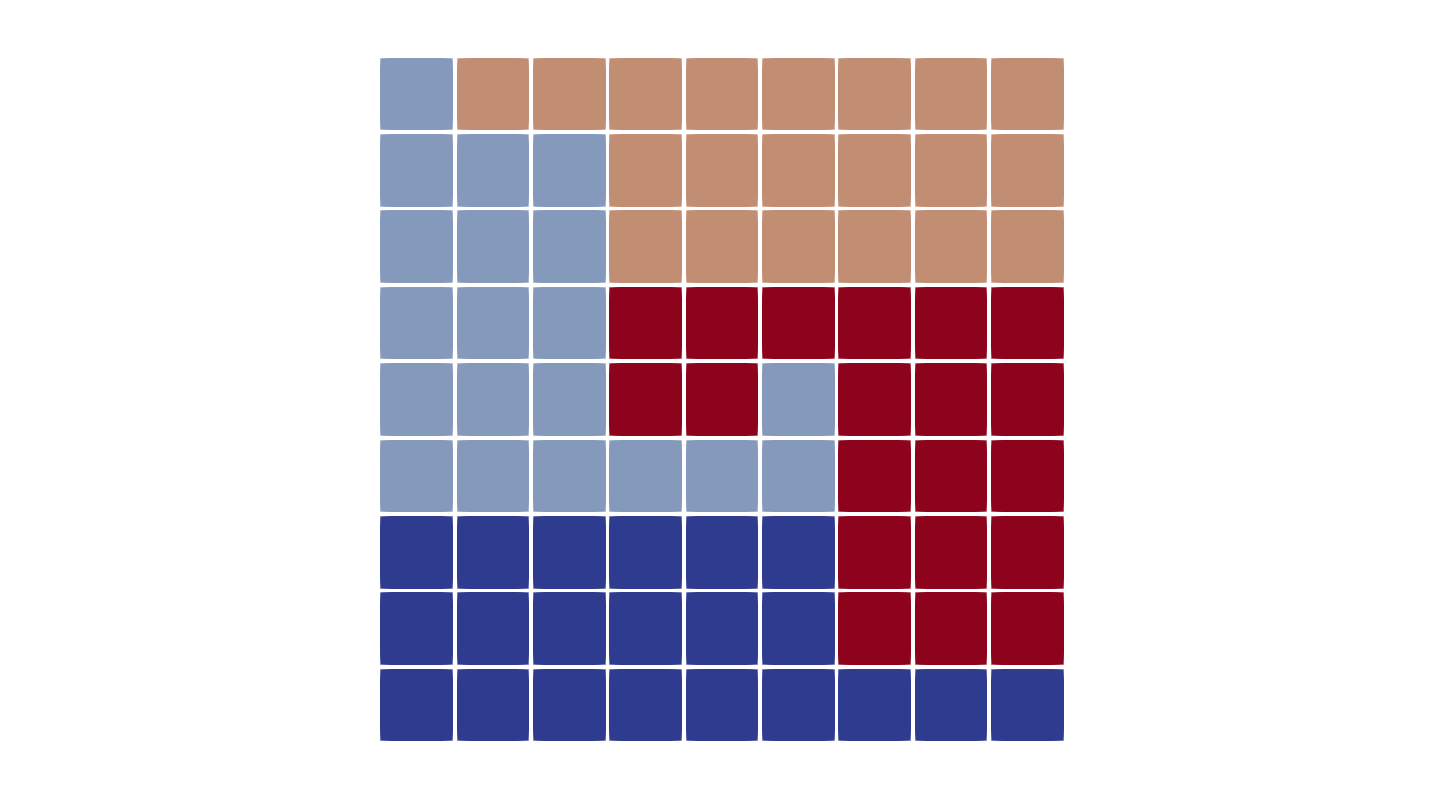
\includegraphics[width=0.54\textwidth]{60_exahype/domain-decomposition.png}
 \end{center}
 \caption{
  Domain decomposition in \ExaHyPE\ for a run with four threads/ranks. Each
  individual cell hosts a patch.
 }
\end{figure}


I plan to support multiple different dynamic load balancing schemes over time,
but the straightforward decomposition scheme shipped with \Peano\ at the moment
is recursive subdivision, a modification of OpenMP's guided scheduling.
To use it, you have to call
\begin{code}
project.set_load_balancing( "toolbox::loadbalancing::RecursiveSubdivision" )
\end{code}

\noindent
on your \ExaHyPE\ project. There are (optional) arguments to this call that
configure the load balancing.
\ExaHyPE\ has its own default configuration. 
Via

\begin{code}
project.set_load_balancing("toolbox::loadbalancing::RecursiveSubdivision", 
 "new ::exahype2::LoadBalancingConfiguration()" )
\end{code}

\noindent
you switch to this default.
You can tailor it further.
With

\begin{code}
project.set_load_balancing(
 "toolbox::loadbalancing::RecursiveSubdivision", 
 "new ::exahype2::LoadBalancingConfiguration(0.8,200)" )
\end{code}

\noindent
for example, you instruct the load balancing that you want it to be well-balanced 
accross ranks up to 80\% (the default is 90\%) and you also to constrain the tree (subpartition) size 
by 200 cells.
This means that no domain on a rank will be split if this rank's load is $\pm20\%$ off, and a partition
will never split up if it has less than 200 cells.

\begin{remark}
 There is a always a trade-off between the different settings: 
 If you increase the quality of the domain decomposition, then the time per time step will go down.
 However, the load balancing will need way longer. 
 If you pick a minimum cell size, then the grid will build up first until it can accommodate the constraint, and then it will decompose.
 Grid decomposition however is both time consuming and requires (temporarily) quite a lot of memory.
\end{remark}   
 



\paragraph{Task parallelism}

Some \ExaHyPE\ solvers add further task parallelism to this decomposition. 
In general, the enclave solvers tend to perform better on massively parallel
systems.



\paragraph{Load balancing settings}

\begin{remark}
 Consult the troubleshooting FAQs in Chapter \ref{chapter:troubleshooting}.
\end{remark}

\noindent
While \ExaHyPE\ makes it relatively straightforward to parallelise a code, 
the tuning of a particular experiment is often tricky.
As \ExaHyPE\ is an engine supporting multiple application (domains) and as the
``perfect'' load balancing strategy depends strongly on the application type
plus the chosen experiments plus the machine used, it can only provide vague
heuristics of settings that work in most of the cases. 
To get really good performance, you will have to play around with the load
balancing settings.


Here are some recommendations if you use the recursive load balancing.
The recommendations describe how to tweak the three parameters that the
\ExaHyPE\ configuration offers:


\begin{itemize}
  \item Do not set the load balancing quality too high. I am usually fine if the
  balancing between the ranks is about 80\%--90\% accurate. 
\begin{code}
project.set_load_balancing(
 "toolbox::loadbalancing::RecursiveSubdivision", 
 "new ::exahype2::LoadBalancingConfiguration(0.8)" )
\end{code}
  First get something up and running and test it. After that, you might want to
  increase the quality closer to 100\%. However, the higher this quality
  threshold the longer your grid setup and balancing time.
  \item Do not set a minimum
  tree size initially.
  Prescribing a number of cells that a subpartition has to have is a powerful tool to ensure that the overhead
  does not become excessive. However, a threshold massively slows down the grid
  construction. So it is better to use this parameter as the last one (see
  below):
\begin{code}
project.set_load_balancing(
 "toolbox::loadbalancing::RecursiveSubdivision", 
 "new ::exahype2::LoadBalancingConfiguration(0.8,0)" )
\end{code}
  \item If your code tends to hang in MPI (consult Chapter
  \ref{chapter:troubleshooting} please), try to kick the simulation off with
  only one partition per rank:
\begin{code}
project.set_load_balancing(
 "toolbox::loadbalancing::RecursiveSubdivision", 
 "new ::exahype2::LoadBalancingConfiguration(0.8,0,1)" )
\end{code}
  Once this passes through, increase the last counter to at most the number of
  cores per rank. As long as you use an enclave-based FV solver, restricting the
  number of subpartitions per rank does not constrain your shared memory
  efficiency too much. It simply means that domain decomposition is not used too
  aggressively to get BSP-type parallelism. Instead, \Peano\ will try to use
  tasks on a per-patch basis.
  \item If you work without periodic boundary conditions, the initial load
  balancing will likely be poor if the mesh is too shallow: The code cannot
  deploy cells along the periodic boundary to other ranks. These always have to
  be handled by rank 0. So it makes sense to set the minimal mesh size (second
  argument) to at least $3^d+1$. This prolongs the load distribution
  sufficiently long until enough cells are available. The knock-on problem then
  is that we have a lot of cells and the load balancing tries to split them up
  evenly---unaware that all the boundary cells can't be distributed. So you will
  have to restrict the number of cells per inter-rank balancing. I recommend to
  to add $3^d$ as fourth argument to \ExaHyPE's load balancing configuration.
  \item If your code suffers from the fact that the load balancing moves around
  too large trees between ranks, use the fourth argument to restrict this
  behaviour.
\end{itemize}


\paragraph{Writing your own parallel extensions}

Most users that write extensions to \ExaHyPE\ which need some global data
exchange are users which add new fields to their solver. Examples are global
statistics that they want to track over the solution or global variables that
they control.

\begin{definition}
 Each MPI rank holds one instance of the solver. 
 All threads per MPI rank share the same instance of the solver.
\end{definition}


\noindent
\Peano\ splits up the domain into chunks along the space-filling curve. 
If you use an enclave solver, it then splits up these chunks further into tasks.
That is, operations per cell such as the Riemann solves and the patch
postprocessing can run in parallel on each thread.

If you add new attributes to your solver, this attribute exists on each solver
on each rank. 
You therefore have to 
\begin{itemize}
  \item ensure that no two threads access the attribute at the same time;
  \item ensure that the attributes of the individual solver instances per rank
  remain consistent.
\end{itemize}

\noindent
The first item is relatively simple: You might, for example, decide to protect
all accesses to your own variables via a semaphore. 
These techniques are discussed in Section
\ref{section:parallel-programming:shared-mem:protect}.
There is no specific place to take care of the protection: 
Just protect the actual data access.


The second item requires slightly more work, as you have to globally reduce the
attribute: After each time step, you have to ensure that all ranks exchange
their attributes with each other, and you then have to merge these data.
I recommend not to use MPI's data exchange routine directly, but to use \Peano's 
wrappers around these routines. 
These wrappers are discussed in Section
\ref{section:parallel-programming:shared-mem:reductions}.
The actual data exchange should be done at the end of a each time step. 
For this, you add
\begin{code}
  void finishTimeStep() override;
\end{code}
to your solver. The implementation should first invoke the superclass
and then add the additional data exchange.
\begin{code}
void mynamespace::MyFancySolver::finishTimeStep() {
  MyFancyAbstractSolver::finishTimeStep();
  #ifdef Parallel
  // additional data exchange
  #endif
}
\end{code}



\ExaHyPE\ internally realises these two steps for all of its solver attributes
such as the maximum mesh size or the admissible time step sizes.


\subsection{Adding adaptive mesh refinement (AMR)}


\begin{remark}
 AMR is application- and numerics-specific. Therefore, the signatures of the
 routines discussed below might change if you switch from Finite Volumes to
 ADER-DG, e.g. The discussed principles however always are the same.
\end{remark}


By default, \ExaHyPE\ solvers operate on a regular grid.
To facilitate an adaptive mesh, you have to ensure that your solver is aware that you operate 
with different $h_{\text{max}}>h_{\text{min}}$. 
So you have to alter these two flags of your solver instantiation.
As \Peano\ operates with three-partitioning, you have to pick 
$h_{\text{min}} \leq \frac{1}{3} h_{\text{max}}$ to switch on adaptivity.

Once AMR is, in principle enabled, you still have to supplement a refinement and/or coarsening criterion:



\paragraph{Supplementing the refinement criterion}
%
On the Python side, dynamic adaptivity is added via a one-liner:

\begin{code}
mysolver.set_implementation(
 refinement_criterion=exahype2.solvers.fv.PDETerms.User_Defined_Implementation 
)
\end{code}


\noindent
Once you did rerun your Python script, you have to add your solver a new
routine:

\begin{code}
::exahype2::RefinementCommand refinementCriterion(
  const double * __restrict__ Q,
  const tarch::la::Vector<Dimensions,double>&  volumeCentre,
  const tarch::la::Vector<Dimensions,double>&  volumeH,
  double                                       t
) override;
\end{code}


\noindent
If this is the first time you create your solver, \ExaHyPE\ adds this routine
into the solver blueprint.
If you add AMR to an existing solver, you have to add the routine manually, as
\ExaHyPE's code generator never overwrites a user solver.
A simple default implementation of this routine resembles

\begin{code}
::exahype2::RefinementCommand MyClass::refinementCriterion(
  const double * __restrict__ Q, // Q[5+0],
  const tarch::la::Vector<Dimensions,double>&  volumeCentre,
  const tarch::la::Vector<Dimensions,double>&  volumeH,
  double                                       t
) {
  ::exahype2::RefinementCommand result = ::exahype2::RefinementCommand::Keep;
  return result;
}
\end{code}


\noindent
This version does not (yet) any adaptivity. 
Your solver returns \texttt{Keep} all the time, so \Peano\ will create a mesh
that just matches $h_{\text{max}}$ as specified via the solver and then keep
this match.
Once you return \texttt{Refine}, it will however refine.
If your mesh however becomes finer than your solver's $h_{\text{min}}$, \Peano\
will ignore the refinement request of your \ExaHyPE\ solver.


\texttt{Keep} keeps the mesh as it is.
That is, if you return \texttt{Keep} for an adaptive grid part, this part will
not change.
You have to invoke \texttt{Erase}\footnote{I chose erase deliberately and not
coarsen, as coarsening has different semantics in multiscale/multigrid
algoritms where coarsening does not remove mesh entities but ``changes the
resolution view''.}.
Both erase and keep are only recommendations to \Peano---\Peano\ will try to
meet these requests, but will always make the mesh slightly finer or not refine
if the minimum mesh size would be violated too harshly.
That is, if some parts of the mesh ask for a refinement and direct neighbours
want to coarsen, the refinement gets higher priority.
Along the same lines, erase instructions will simply be ignored if the resulting
mesh would be coarser than $h_{\text{max}}$.


\begin{remark}
It is important to keep in mind that refinement requests are not
immediately realised by \Peano. 
Refinements are requested in one time step, and then realised in the subsequent
one.
Also, \Peano\ will try to accommodate coarsening requests, but if there are any issues (with mesh partitioning or balancing, e.g.), then these
considerations willl have higher priority and \Peano\ might decide to continue with a finer mesh than requested.
\end{remark}


\noindent
Different solvers come along with different interpolation and restriction seems.
The discussion around Finite Volume solvers for example can be found on page
\pageref{section:exahype:finite-volumes:interpolation-schemes}.


\subsection{GPU support}

\begin{definition}
 \ExaHyPE\ uses GPUs in a classic \emph{offloading, accelerator style}.
 This means that it takes particular tasks, ships them to the GPU and then ships
 them back. 
 This happens under the hood, and neither does data reside on the accelerator
 permanently nor is the accelerator used all the time.
 
 The whole approach assumes that there are computations (cell/patch updates)
 which can be done without any effect on global variables. 
 It works if and only if we can ship a task to the GPU, and then get the
 solution data for this task back and no other global variabled changes.
 We furthermore assume that the computations that fit onto the GPU have no
 state.
 They can use some global, static variables, but they cannot access the solver's
 state which can change over time. 
 We rely on code parts with \emph{have no side effects and do not depend on
 the solver state} (minus global variables).
 
 This might not work for all patches: There are always patches which evaluate
 and analyse some global data, or build up global data structures. 
 In this case, \ExaHyPE\ only offloads the remaining, simple patches to the GPU. 
\end{definition}


\noindent
\ExaHyPE\ supports GPUs via task offloading.
To use GPUs, you have to follow the following steps:





\paragraph{First, your environment has to be compiled with GPU support.}
For this, configure with the argument \texttt{--with-gpu} and select an
appropriate GPU programming model.
There is a brief discussion on this in Section
\ref{section:installation:configure}.
Rebuild the whole \Peano\ core.

\begin{remark}
 If you want to profile or optimise your code, you might want to pick a
 particular vendor toolchain. See configure's help on \texttt{--with-toolchain}.
\end{remark}



\paragraph{Second, use an \ExaHyPE\ solver which has support for GPUs and instruct
it that you plan to have patch updates without access to the solver's
internal state.}
The Finite Volume enclave solvers for example all support GPUs, but the
versions without enclave tasking do not support them.
The solver documentation should clarify which one to select.
For most of these GPU-enabled solvers, it is sufficient to pass an additional
flag (\texttt{pde\_terms\_without\_state=True} for the FV variants, e.g.)
that tells the solver that we have PDE terms which have no side effect which
also do not need the solver object.


\paragraph{Third, provide the additional PDE terms without state.}
%
%
To faciliate the offloading, we have to create alternative versions of our PDE
term functions that can work independent of the solver object (and in return
cannot modify it).
Depending on which terms we have, we'll need stateless versions of the flux, the
non-conservative product and the source term. 
We'll always needs the eigenvalue function. 
Per function, keep the original one and add a second one which is 

\begin{itemize}
  \item static;
  \item accepts an additional flag of type \texttt{Offloadable}. This is the last argument, i.e.~a static
  version of a function has exactly the same arguments as the non-static,
  default variant but then has one more argument. The last argument is solely
  there to be able to distinguish the static version from the normal one, as C++
  cannot overload w.r.t.~static vs.~not static. \texttt{Offloadable} is
  automatically defined in the abstract base class which \ExaHyPE's Python API
  generates.
  \item is embedded into 
\begin{code}
#if defined(OpenMPGPUOffloading)
#pragma omp declare target
#endif

my new static function variants

#if defined(OpenMPGPUOffloading)
#pragma omp end declare target
#endif
\end{code}
  Though you can leave these annotations away if you use SYCL only.  
\end{itemize}

\noindent
Very often, the standard flux and eigenvalue routines can invoke the
static variants and you can thus eliminate code redundancies.
For example, you might have the normal flux function and a static flux function
with the additional \texttt{Offloadable} parameter, but the 
normal function just invokes the static cousin.

In many of our codes, we take a function like
\begin{code}
void examples::exahype2::SSInfall::SSInfall::flux(
 ...
)  {
  logTraceInWith4Arguments( "flux(...)", faceCentre, volumeH, t, normal );
  assertion4( Q[0]>0.0, faceCentre, volumeH, t, normal );
  compute something;
  assertion4( F[0]>0.0, faceCentre, volumeH, t, normal );
  logTraceOutWith4Arguments( "flux(...)", faceCentre, volumeH, t, normal );
}
\end{code}

\noindent
and simply split it into two variants:
\begin{code}
void examples::exahype2::SSInfall::SSInfall::flux(
 ...
)  {
  logTraceInWith4Arguments( "flux(...)", faceCentre, volumeH, t, normal );
  assertion4( Q[0]>0.0, faceCentre, volumeH, t, normal );
  flux(Q,faceCentre,volumeH,t,normal,F,Offloadable::Yes);
  assertion4( F[0]>0.0, faceCentre, volumeH, t, normal );
  logTraceOutWith4Arguments( "flux(...)", faceCentre, volumeH, t, normal );
}


void examples::exahype2::SSInfall::SSInfall::flux(
  ...,
  Offloadable
)  {
  compute something;
}
\end{code}


\noindent
The static version is used on the GPU. 
The normal one is used on the CPU yet defers immediately to the static version.
Please note that GPUs are quite restrictive w.r.t.~terminal outputs and
assertions.
You will have to remove both from your static routine versions.
In the example above, the non-static version wraps the core functionality into
assertions. 
Therefore, we have the assertions on the CPU, but the core part that goes to the
GPU is free of assertions.
The same holds for the logging.


\paragraph{Finally, pick a threading backend which supports GPU offloading.}
%
%
%
The default threading model of \Peano\ does not support task fusion or the
offloading to GPUs. 
If you run the code with \texttt{--help}, it will report on various threading
models.
Use one that has \texttt{fuse} in its title, and you should finally get GPU
offloading.




\begin{remark}
 If only some patches/cells can be offloaded to the GPU, then you can redefine
 the routine
 \begin{code}
virtual bool patchCanUseStatelessPDETerms(
  const tarch::la::Vector<Dimensions,double>&  patchCentre,
  const tarch::la::Vector<Dimensions,double>&  patchH,
  double                                       t,
  double                                       dt
) const;
 \end{code} 
 
 \noindent
 in your
 solver. By default, this routine returns \texttt{true} always. Here's the clue: 
 This is a normal function, i.e.~you can use the solver's state and make the
 result depend on this one.
\end{remark}


\section{Finite Volume extensions}


\subsection{Boundary conditions}


Boundary conditions often are tricky to implement and solely up to the user. 
In \ExaHyPE, Dirichlet and Neumann boundary conditions on Cartesian meshes are
close to trivial.
More sophsticated boundary conditions require slightly more work. 
Here are some remarks how to implement them.


\begin{remark}
  The boundary condition semantics are solely determined by the user's boundary
  condition callback.
  Therefore, it is possible to use different boundary conditions in different
  domain areas.
\end{remark}


\begin{figure}[htb]
 \begin{center}
  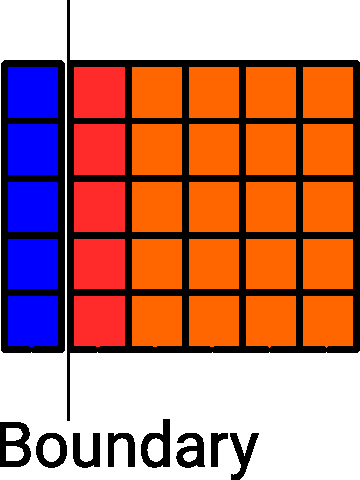
\includegraphics[width=0.2\textwidth]{60_exahype/boundary.pdf}
 \end{center}
 \caption{
  \ExaHyPE's Finite Volume scheme organises its mesh into patches. 
  Here, we use a 5$\times $5 patch (orange/red).
  Prior to the update of a patch, \ExaHyPE\ calls \texttt{boundaryConditions}
  for each of the volumes adjacent to the boundary (darker red).
  The routine allows you to alter the value of the halo surrounding the patch
  (blue).
  The outer (blue) cells are subsequentially used to determine a flow through
  the boundary into the domain.
  \label{figure:exahype:boundary-conditions}
 }
\end{figure}

\noindent
Boundary conditions in general are realised via their own callback called
\texttt{boundaryConditions}.
When you run the Python toolkit, you get an empty implementation of this routine
that you can befill.
The routine is called per outer volume (Figure
\ref{figure:exahype:boundary-conditions}).



\paragraph{Dirichlet boundary conditions}.
%
%
%
Dirichlet boundary conditions 
\[
  Q(x) | _{\partial \Omega } = f(x,t)
\]
are close to trivial to implement. 
You set  outer values due to

\begin{code}
void ...::MySolver::boundaryConditions(
  ...
) {
  Qoutside[0] = ...
  Qoutside[1] = ...
  ...
}
\end{code}

\noindent
Obviously, the values on the right-hand side can depend on time and spatial
position.
We find two different ways to impose Dirichlet conditions:
\begin{enumerate}
  \item You simple set the outer volumes (blue in Figure
\ref{figure:exahype:boundary-conditions}) to $f(x,t)$.
  \item You compute the average between the blue value and the interior value as
  $Q | _{\partial \Omega } = \frac{1}{2} (Q_{\text{outside}} +
  Q_{\text{inside}}) = f(x,t)$ which yields $Q_{\text{outside}} =
  2f(x,t)-Q_{\text{inside}}$.
\end{enumerate}

\noindent
The latter formula is inspired by Finite Differences and might give a slightly
more accurate values.
With a sole averaging Riemann solver, it directly sets the flux.
If you use something like Rusanov, you might tweak $Q_{\text{outside}}$ further
such that the eigenvalue term along the boundary face has the correct
(imposed) value too.


\paragraph{Neumann boundary conditions (Finite Volumes)}

As we can read the volume values inside the domain prior to a time step
and modify those outside of the domain, it is straightforward to implement
homogeneous Neumann conditions.
The snippet below implements homogeneous Neumann conditions

\[
  \left( \nabla Q(x), n \right)  | _{\partial \Omega } = 0
\]


\begin{code}
void ...::MySolver::boundaryConditions(
  ...
) {
  Qoutside[0] = Qinside[0];
  Qoutside[1] = Qinside[1];
  ...
}
\end{code}

\noindent
but obviously you can use a simple Finite Differences scheme to impose
non-homogeneous conditions as well.



\paragraph{Inflow/outflow boundary conditions}

Inflow or outflow boundary conditions are conceptually close to Neumann
conditions. 
Often, it is however reasonable to supplement them with some limiter, i.e.~if
the flow is close to zero and inwards, a modified outflow condition could
manually set it (limit it) to zero.


While this approach does work in most of the cases, it struggles to handle
information flow that is not orthogonal to the Cartesian faces.
It assumes that all flow is axis-aligned:
You can only modify the face-connected neighbour volume in the ghost 
region outside of the domain.
You cannot alter diagonal volumes.
Unless you want to use distorted, i.e.~boundary-aligned, meshes as discussed
below, there's no way around this.
Yet, increasing the domain size usually helps in such a case.




\paragraph{Extrapolating boundary data (Finite Volumes)}



It is more complicated to realise boundary conditions that extrapolate
data into the outside.
Such boundary conditions read as
\[
  Q(x) | _{\partial \Omega } = \lim _{x \mapsto \partial \Omega}
  f(Q(x,t),\nabla f(Q(x,t))
  \ \text{or} \
  \left( \nabla Q(x), n \right) | _{\partial \Omega } = \lim _{x \mapsto
  \partial \Omega} f(Q(x,t),\nabla f(Q(x,t)).
\]
It is obviously trivial to extrapolate the solution value within the domain to
the boundary volumes (dark red to blue value in Figure
\ref{figure:exahype:boundary-conditions}), but once you need the derivatives at
the boundaries, you have to invest more work.
After all, the boundary routine only provides access to the boundary data, but
not to any derivatives.


Users have successfully implemented non-homogeneous Neumann boundary
conditions where they extrapolate the derivatives onto the boundary and use
those to inform the actual value.
This requires work however:

\begin{itemize}
  \item Introduce a new material parameter that stores the directional
  derivative. If you need the non-homogeneous Neumann conditions all around the
  domain, you will need \texttt{Dimensions} material parameter per unknown:
  \begin{code}
mySolver = MySolver( "Myname", my_patch_size, number_of_unknowns,
  auxiliary_variables=3*number_of_unknowns, ... );
  \end{code}
  \item Compute the derivatives per volume after each time step in a Finite
  Differences sense. We can add such a code snippet in Python:
  \begin{code}
my_solver.preprocess_reconstructed_patch_kernel = """
  dfor(cell,patchSize) {
    //tarch::la::Vector<Dimensions,int> currentPosition=marker.getOffset()+(cell+0.5)*volumeH;
    tarch::la::Vector<Dimensions,int> currentCell = cell + tarch::la::Vector<Dimensions,int>(1);

    tarch::la::Vector<Dimensions,int> leftCell  = currentCell;
    tarch::la::Vector<Dimensions,int> rightCell = currentCell;
    leftCell(d)  -= 1;
    rightCell(d) += 1;

    if (cell(0)==0) { // left layer of patch, so use right differences
      const int rightCellSerialised  =
        peano4::utils::dLinearised(rightCell,patchSize + 2*1); 
      const int currentCellSerialised = 
        peano4::utils::dLinearised(rightCell,patchSize + 2*1); 
      for(int i=0; i<unknowns; i++) { 
        target[currentCellSerialised*(unknown+auxiliaryVariables)+i] = 
         1/h * (
           target[rightCellSerialised*(unknown+auxiliaryVariables)+i] -
           target[centralCellSerialised*(unknown+auxiliaryVariables)+i]
         );
  ...
      }}}"""
\end{code}
  \item With this information, we can finally set the boundary conditions:
  The routine \texttt{boundaryConditions} is given the data at the boundary.
  Due to our modifications, these data are augmented by additional ``material''
  parameters\footnote{The term ``material parameter'' implies that they are not
  subject to the flux equations.} which store the derivatives from the current
  time step.
  We can thus realise boundary conditions which use the (boundary-extrapolated)
  derivative besides the actual value.
\end{itemize}



\paragraph{Boundary-aligned geometries}

\ExaHyPE's mesh is topologically Cartesian.
That does not mean that you have to work in a Cartesian world.
You can distort, squeeze, rotate the mesh locally as long as your mesh topology
remains adaptive Cartesian.
Codes like the ExaSeis simulation package introduce material parameters per
degree of freedom to encode mesh distortions.
This allows them to represent a boundary exactly, i.e.~to adopt the Cartesian
mesh to the real domain boundaries.
Obviously, the actual boundary condition implementations then have to be adopted
accordingly, too.








\subsection{Interpolation and restriction schemes}
\label{section:exahype:finite-volumes:interpolation-schemes}

If you employ adaptive mesh refinement, you have to project coarser resolutions
onto finer resolutions (interpolation), and you have to couple back fine grid
solutions to coarser regions of the mesh (restriction).
By default, all \ExaHyPE\ Finite Volume solvers employ a piece-wise constant
interpolation and simple averaging as restriction.
If you require a better inter-grid transfer scheme or if you want to introduce your own one, you have to do the following steps:

\begin{itemize}
  \item Make your solver (in Python) use another interpolation scheme. I present
  a variant here where you want to use linear interpolation:
  \begin{code}
my_solver._action_set_couple_resolution_transitions_and_handle_dynamic_mesh_refinement.
  switch_interpolation_scheme( "linear" )
  \end{code}
  \item For a different restriction scheme use the routine
  \texttt{switch\_interpolation\_scheme()}.
  \item Call the solver's \texttt{create\_action\_sets()}. If you omit this
  call, your switch of the scheme is not ``committed'', i.e.~taken into account
  (though subsequent changes of the solver state might in turn call
  \texttt{create\_action\_sets()} and thus implicitly make your switch known to
  the class).
  \item Depending on your Finite Volume scheme, you might have to change the
  size of the halo layer. The Rusanov solvers for example all work with a halo
  layer of 1. They don't need larger overlaps between neighbouring volumes, as
  the Rusanov Riemann solver only needs the solution left and right of a face.
  If you want to use a higher-order interpolation however, you need larger
  overlaps. In this case, you have to extend the halo layer used:
  \begin{code}
my_solver.overlap=2
  \end{code}
\end{itemize}


\paragraph{Realisation and available schemes}
%
%
All the interpolation and restriction schemes that we offer can be found in the
file \texttt{toolbox/blockstructured/Interpolation.h}.
The documentation within this file\footnote{We recommend to run
\texttt{doxygen} on the sources as discussed in Section
\ref{section:installation:documentation} and then to use a webbrowser to study
the documentation. The interpolation/restriction details are discussed on a 
separate page which you find when you click on ``Related Pages'' within the
generated webpage.} explains how the actual realisations work.
\ExaHyPE's philosophy is that you implement the inter-grid transfer operators
within this header, and the Python API then helps you to pick from the routines
therein.

At the moment, we have only implemented \texttt{averaging} for the restriction. 
For the interpolation, we offer the following routines:

\begin{center}
 \begin{tabular}{l|p{8cm}}
  {\bf scheme} & description \\
  \hline
  \texttt{piecewise\_constant} & Interpolate piece-wise constant (default) \\
  \texttt{linear\_with\_constant\_extrapolation} & Interpolate linear (2d) or
  bi-linear (3d) along faces and use constant extrapolation along diagonals and
  patch boundaries.
  \\
  \texttt{linear\_with\_linear\_extrapolation} & Interpolate linear (2d) or
  bi-linear (3d) along faces and use constant extrapolation along diagonals and
  patch boundaries.
  \\
  \texttt{linear\_with\_constant\_extrapolation\_and\_linear\_normal\_interpolation}
  & Variation of \texttt{constant\_with\_constant\_extrapolation} where we
  interplate linearly between restricted (coarsened) voxel data and the adjacent real
  coarse grid values. 
  \\
  \texttt{linear\_with\_linear\_extrapolation\_and\_linear\_normal\_interpolation}
  & Variation of \texttt{linear\_with\_constant\_extrapolation} 
  \\
 \end{tabular}
\end{center}


\paragraph{Postprocessing}
%
%
%
Some codes need to postprocess their interpolation data. At the moment, I only support volume-wise postprocessing.
To enable it, you pass a function call to the DynamicAMR argument: 
\begin{code}
my_solver._action_set_couple_resolution_transitions_and_handle_dynamic_mesh_refinement.
  switch_point_wise_postprocessing_of_interpolation("""
  targetVolume[0] = 0.1;
  targetVolume[1] = 0.1;
  targetVolume[2] = std::max(targetVolume[2],0.0);
  """ )
\end{code}

\noindent
Alternatively, just invoke a function directly:

\begin{code}
my_solver._action_set_couple_resolution_transitions_and_handle_dynamic_mesh_refinement.
  switch_point_wise_postprocessing_of_interpolation(
  "examples::exahype2::ccz4::enforceCCZ4constraints(targetVolume)" )
\end{code}

\noindent
With this variant, you trigger the interpolation of your choice, and, after
that, each individual volume is subject to a function
\texttt{enforceCCZ4constraints} which might change the value.
As this \texttt{enforceCCZ4constraints} in this example is user-defined,
\ExaHyPE's core routines cannot know its definition.
We manually have to add an include:

\begin{code}
my_solver._action_set_couple_resolution_transitions_and_handle_dynamic_mesh_refinement.
 additional_includes += """ 
   #include "../CCZ4Kernels.h"
 """
\end{code}

%  \item Make your solver (in Python) use another interpolation scheme. I
%  % present a variant here where you want to use linear interpolation:
%  \begin{code}
%self._action_set_couple_resolution_transitions_and_handle_dynamic_mesh_refinement.additional_includes
% += """ #include "../CCZ4Kernels.h"
%"""
%#
% self._action_set_couple_resolution_transitions_and_handle_dynamic_mesh_refinement.switch_restriction_scheme( "averaging" ) self._action_set_couple_resolution_transitions_and_handle_dynamic_mesh_refinement.switch_interpolation_scheme( "linear" )
%  \end{code}


\noindent
\texttt{targetVolume} is a double pointer to the volume that has been interpolated.
There are a few more values available for any function call you wanna make, but
the pointer to the quantities usually is the most important one.
You can use the attribute \texttt{additional\_includes} to give the resulting
source code access to other routines.



\section{Modelling the fluxes and Riemann solvers with SymPy}

You can model your fluxes, Riemann solvers and so forth with SymPy, 
i.e.~through symbolic formulations---as long as you use a generic numerical
Riemann solver such as Rusanov.
The \ExaHyPE\ SymPy wrapper is
held within the \ExaHyPE\ subpackage \texttt{exahype2.sympy}.


I provide a couple of classes for different PDE variants that should be
compatible to particular \ExaHyPE\ Finite Volume and ADER-DG solvers.
All SymPy classes wrap around SymPy's symbolic expressions, and thus allow users
to work with these expressions directly.
Once you have finished you modelling, the wrappers offer some code generation
which again decorate SymPy's code generation, adds some glue code and can inject
the generate into a \Peano\ solver.


The Euler equations modelled via this interface then add the following code
snippet to the Python script that models \Peano:

\begin{code}
import sympy
import exahype2.solvers.sympy.FirstOrderConservativePDEFormulation


#
# Create a new instance of symbolic ExaHyPE PDE interface.
#
pde = exahype2.solvers.sympy.FirstOrderConservativePDEFormulation(unknowns = 5,dimensions = 3)

#
# Give entries in input vector symbolic names. We first declare some
# helpers/constants. Then we tell the solver how we would like to name the Q 
# entries
#
gamma = sympy.symbols( "gamma")
rho   = pde.name_Q_entry( 0, "rho" )
j     = pde.name_Q_entries( 1, 3, "j" )
E     = pde.name_Q_entry( 4, "E" )

#
# Finally, define the equation system
#
p = (gamma - 1 ) * (E-1/2 * exahype2.solvers.sympy.dot(j,j) / rho)

pde.F[0,:]   = j
pde.F[1:4,:] = 1/rho * exahype2.solvers.sympy.outer(j,j) + p * sympy.eye(3)
pde.F[4,:]   = 1/rho * j * (E+p)

c = sympy.sqrt( gamma * p /rho )
pde.eigenvalue[0] = [ j[0]/rho - c, j[1]/rho - c, j[2]/rho - c ]
pde.eigenvalue[1] = [ j[0]/rho, j[1]/rho, j[2]/rho ]
pde.eigenvalue[2] = [ j[0]/rho, j[1]/rho, j[2]/rho ]
pde.eigenvalue[3] = [ j[0]/rho, j[1]/rho, j[2]/rho ]
pde.eigenvalue[4] = [ j[0]/rho + c, j[1]/rho + c, j[2]/rho + c ]

pde.substitute_expression( gamma, 1.4 )
\end{code}


\noindent
This \texttt{pde} object here can create C++ code that we can plug directly into
the respective \Peano\ routines:
\begin{code}
my_solver.set_implementation( flux=pde.implementation_of_flux(),eigenvalues=...
\end{code}

\noindent
With this call, the modelled PDE feeds, via code generation, directly into the
\ExaHyPE\ solver. When we remodel the PDE, everything is updated automatically.


If you study the interface of \texttt{set\_implementation}, you will notice that
you can also model boundary or initial conditions this way.
In this example, we however only modelled flux and eigenvalues.
The remaining callbacks remain plain C++.


For further resources, please visit SymPy's homepage, and maybe you also want to
have a look into projects like EinsteinPy or galgebra which provide tools for
astrophysics or geometric algebra, respectively.
As we rely on SymPy and expose all the SymPy expressions, they are compatible
with \ExaHyPE.




\section{Adding tracers}

To add tracer support for \ExaHyPE, you first have to reconfigure our run and
add the 
\begin{code}
./configure ... --enable-particles
\end{code}

\noindent
Adding tracers is fairly simple.
Each tracer has to have a name, and you also have to inform the project how many
attributes you plan to track per tracer:

\begin{code}
tracer_particles = project.add_tracer( name="MyTracer",attribute_count=2 )
\end{code} 


\begin{remark}
 Study the in-code documentation of the involved classes. 
 Tracers can track only some attributes, they can move or stay at one place,
 and they can also interact with each other. 
\end{remark}


\noindent
This prepares \ExaHyPE\ to handle your tracer, and it also dumps tracers already
with each snapshot, but obviously you haven't inserted any tracers yet. 
There are different inserters shipped with \ExaHyPE. 
Alternatively, you might want to write your own, bespoke particle seed (see
below).
The snippet below inserts particles into your grid along a Cartesian topology
and adds some random noise:


\begin{code}
project.add_action_set_to_initialisation( 
 exahype2.tracer.InsertParticlesAlongCartesianMesh( 
  particle_set=tracer_particles,
  h=args.h/8.0, noise=True 
))
project.add_action_set_to_timestepping(
  peano4.toolbox.particles.UpdateParallelState(
    particle_set=tracer_particles
  )
)
\end{code}


\begin{definition}
 All of \Peano's particle toolbox routines are written for large-scale
 parallel (MPI) runs.
 Therefore, you have to add \texttt{UpdateParallelState} to the time stepping
 always.
\end{definition}

\noindent
With this additional seed and the update of the particle state, you can run your
code and visualise the particles.
However, these particles do not move at all yet or track the actual data of
interest.
To facilitate this, you have to map your solution onto the particle first.
Let \texttt{thesolver} be your \ExaHyPE\ solver instance in the Python script.
Not all solvers currently support tracers (efficiently), but we are continuously
improving the tracer support.
With the solver instance and the tracers, we can couple the two ingredients.
You have to pick different coupling schemes depending on the type of your
solver:

\begin{code}
project.add_action_set_to_timestepping(
  exahype2.tracer.FiniteVolumesTracing(
    tracer_particles,
    thesolver,
    [],        # velocity indices
    range(59), # data indices
    0,         # scaling of velocities
    time_stepping_kernel="toolbox::particles::StaticPosition"))
\end{code}


\subsection{Dump tracer data into CSV database}

The likely most important tool for many developers using only few particles is
the fact that particles can dump their solution into a database:

\begin{code}
project.add_action_set_to_timestepping( 
 exahype2.tracer.DumpTrajectoryIntoDatabase(
  tracer_particles,thesolver,particle_spacing/10.0,"TracerDB"
))
\end{code}

\noindent
Dumping tracers into a (CSV) database is attractive, as these files are easier
to parse/postprocess than mesh data files. 
At the same time, you can dump particles more often than you plot data
snapshots, and these dumps can even be adaptive, i.e.~you dump if and only if a
particle actually moves.
The \texttt{DumpTrajectoryIntoDatabase} documentation provides more detail.


\subsection{Write your own particle seed}

If you want to write your own particle seed, I recommend that you copy over an
existing one and adopt it to your need.
Switch to \texttt{python/exahype2/tracer} and copy the class \linebreak
\texttt{InsertParticlesAlongCartesianMesh} over to modify it.
The invocation within your Python application script then has to be altered,
too:

\begin{code}
project.add_action_set_to_initialisation( MyFancySeed(. ..) ))
\end{code}


\noindent
The core ingredients in the seed is the code snippet that decides what happens
if you touch a vertex for the first time:
\begin{code}
  __Template_TouchVertexFirstTime = jinja2.Template("""
  if ( not marker.isRefined() ) {
    auto newParticles =
    toolbox::particles::createEquallySpacedParticles<globaldata::{{PARTICLE}}>...
    for (auto& p: newParticles) {
      p->setNumber(0,_spacetreeId);
      p->setNumber(1,_particleNumberOnThisTree);
      _particleNumberOnThisTree++;
    }
    fineGridVertex{{PARTICLES_CONTAINER}}.insert( 
      fineGridVertex{{PARTICLES_CONTAINER}}.end(), newParticles.begin(),
      newParticles.end() 
    ); 
  }
""")
\end{code}

\noindent
The routine only triggers some activities for unrefined vertices. 
If a vertex is not refined further, it invokes the routine 
\texttt{createEquallySpacedParticles} from the particle toolbox which
returns a container over particles, and then takes these particles and 
inserts them into the domain.
While you can alter this mechanism obviously, a modified, simpler seed can look
like this:

\begin{code}
  __Template_TouchVertexFirstTime = jinja2.Template("""
  if ( 
    not marker.isRefined() 
    and
    marker.x(0)==...      // check where the centre of this vertex is
    and
    marker.x(1)==...      // check where the centre of this vertex is
    and
    marker.x(1)==...      // check where the centre of this vertex is
    and
    marker.h(0)==...      // check how big the area around this vertex is
    and
    ...
  ) {
    globaldata::{{PARTICLE}}* p = new globaldata::{{PARTICLE}}( ... ); 
    p->setNumber(0,_spacetreeId);
    p->setNumber(1,_particleNumberOnThisTree);
    p->setX(0, ... );     // x coordinate
    p->setX(1, ... );     // y coordinate
    p->setX(2, ... );     // z coordinate
    p->setCutOffRadius(0.0); // you can force particles to certain resolution 
                             // levels. Not used here.
    _particleNumberOnThisTree++;
    fineGridVertex{{PARTICLES_CONTAINER}}.push_back( p ); 
  }
""")
\end{code}





\subsection{Encourage particles to spread out evenly}

You can make particles interact with eac other. 
This allows you, for example, to
realise some SPH on top of the code.
One of the most convenient features is to encourage tracers to align in a
quasi-uniform way, i.e.~they do follow the solution characteristics but at the
same time try to space out evenly.
This is allowed via a modified, inverted Lennard-Jones potential
which is parameterised with a distance.
If two particles are closer than that distance, they repulse each other. 
If they are further away than that distance, they attract each other.

\begin{code}
project.add_action_set_to_timestepping( peano4.toolbox.particles.ParticleParticleInteraction(
  particle_set = tracer_particles,
  cell_compute_kernel = exahype2.tracer.perserveCartesianTracerLayout(thesolver,particle_spacing),
  additional_includes = """
#include "repositories/SolverRepository.h"
#include "toolbox/particles/potentials/Springs.h"
"""
))
\end{code}

\noindent
There are further particle-particle interaction scripts in the repository.


\subsection{Changing the grid-to-particle interpolation and/or time stepping}

Most tracing routines (like the \texttt{exahype2.tracer.FiniteVolumesTracing}
above) rely on an interpolation kernel which takes the PDE solution and maps 
some quantities from there onto the tracer and then performs the actual time
stepping.
While the mapping glue code is configured via Python, the actual interpolation
and time stepping are realised via C++ in the particles toolbox.


If you want to add another mapping and/or time stepping, I recommend that you 
extend \texttt{src/toolbox/particles/Tracer.h}:
Insert a new routine for the interpolation there which has exactly the same
signature as \texttt{mapParticleOntoVoxel} and then pick this new routine
through the Python API.




% \section{Ghoddess DG solvers}
% % 
% % We also do provide an interface to Ghoddess DG solvers.
% % Ghoddess solvers use a classic DG formulation with explicit time stepping.
% % Their big USP within \ExaHyPE\ is they rely on a quasi-symbolic formulation and
% % thus facilitate even fast prototyping.
% % 
% \begin{remark}
%   This yet has to be written.
% \end{remark}
 


% \section{Introducing a new numerical scheme}
% 
% This section discusses how to introduce a totally new numerical solver. 
% It does not discuss how to introduce a new PDE, as new PDEs are built using
% \ExaHyPE, i.e.~you pick a solver and then you tweak your PDE terms. 
% That's the thing \ExaHyPE\ is built for and the standard usage model.
% This section gives you an idea how to extend the \ExaHyPE\ core instead,
% i.e.~how to implement a new solver type with different PDE terms, e.g., or a
% type that is more restrictive but particularly optimised.
% 
% \begin{remark}
%   \ExaHyPE\ is a very high level Python API which generates a \Peano\
%    Python project which in turn creates the ``real'' \Peano\ C/C++ code. If you
%    introduce a new numerical scheme/solver to \ExaHyPE, you thus might want to
%    familiarise yourself with \Peano's Python API and how to extend it. This
%    recommendation affects all the gluecode/framework aspects of the software.
%    All the core numerics of \ExaHyPE\ are held as C++ code in the
%    \texttt{src/exahype2} directly and compiled into a separate library. If you
%    introduce new numerical schemes, you might have to extend this library, too.
% \end{remark}
% 
% 
% 
% \subsection{A new Finite Volume solver (native \ExaHyPE)}
% 
% Introducing a new Finite Volume (FV) scheme is reasonably straightforward within
% \ExaHyPE.
% It relies directly on \Peano's patch-based AMR.
% At the moment, I have two flavours of FV available: A single sweep solver which
% runs over the mesh once per time step and the enclave solver which needs two
% sweeps but offloads the majority of the operations onto dedicated tasks.
% 
% 
% \paragraph{Solver base class}
% 
% To start your development, create a new subclass of either \linebreak
% \texttt{exahype2.solver.fv.SingleSweep} or \texttt{exahype2.solver.fv.Enclave}.
% You might want to require the user to specify more constructor arguments, but 
% you need at least those of the superclass.
% 
% 
% 
% \paragraph{The C classes/templates}
% 
% \ExaHyPE's design concept is that each solver yields two types of classes:
% The actual solver and an abstract superclasses. 
% Abstract superclasses are regenerated every time you rerun the Python script.
% Furthermore, they define the whole signature, i.e.~if you alter the signature
% later on, users simply rerun the toolkit. 
% Finally, the abstract superclasses hold default implementations\footnote{Some
% solvers do not expect the user to write any C/Fortran code at all. In this
% case, the solvers nevertheless should create an abstract superclass (now
% holding all functions) and a subclass which is basically empty. This way, we
% are consistent.}.
% 
% 
% Once you have picked either 
% \texttt{exahype2.solver.fv.SingleSweep} or \linebreak
% \texttt{exahype2.solver.fv.Enclave},
% you'll get the four files (two classes) generated.
% However, you might want to tailor these. 
% After all, they do not contain anything that is particular to your domain: 
% They simply hold routines plugging into the steps. 
% To add further functionality, set the fields
% 
% \begin{code}
%   self._abstract_solver_user_declarations  = "..."
%   self._abstract_solver_user_definitions   = "..."
%   self._solver_user_declarations           = "..."
%   self._solver_user_definitions            = "..."
%   self._constructor_implementation         = "..."
% \end{code}
% 
% \noindent
% in your constructor. 
% There are more fields like this. 




% \paragraph{The Python code}
% 
% 
% The core implementation effort clearly has to go into the parts where the actual
% mesh traversal is mapped onto solver calls.
% In \ExaHyPE, this is realised through templates. 
% Any Finite Volume code relies basically on four templates:
% 
% \begin{itemize}
%   \item \texttt{AMRTemplate} will be called on solver cells to determine whether
%   to refine or erase.
%   \item \texttt{AdjustCellTemplate} will be called to impose initial conditions
%   or interior ones.
%   \item \texttt{HandleBoundaryTemplate} is invoked for boundary faces.
%   \item \texttt{HandleCellTemplate} is the actual Finite Volumes solver
%   invocation.
% \end{itemize}
% 
% 
% \noindent
% These four strings are Jinja templates. The idea is that particular FV
% subclasses ``overwrite'' (set) them and thus inject their solver behaviour.
% Each handle is guarded by an additional expression (some C++ code evaluating to
% boolean) to switch it on/off.
% There's two more things that are automatically done: patch updates are
% automatically projected onto the faces, and the projected face data is
% automatically rolled over.
% While these things are ``hard-coded'', you still have guards to switch it
% on/off.
% 
% 
% The template mechanism works similar to aspect-oriented programming, i.e.~it
% simply enables Python to plug some code snippets straight into your the
% generated \ExaHyPE\ code. 
% For a list of predefined constants that are available within the templates,
% please consult the routine
% \texttt{\_init\_dictionary\_with\_default\_parameters} which befills a lookup
% table.
% You can, obviously, add more entries within your implementation.
% For this, a solver has to implement
% \texttt{add\_entries\_to\_text\_replacement\_dictionary}.
% Some of the most important preset dictionary entries are:
% 
% 
% \begin{itemize}
%   \item \texttt{fineGridCell\{UNKNOWN\_IDENTIFIER\}.value} which is a double
%     pointer which points to the whole patch hosted by the cell in the volumetric
%     routines \texttt{CreateCellTemplate}, \texttt{HandleCellTemplate} and
%     \texttt{AMRTemplate}. The array it points to has the size \linebreak
%     \texttt{\{NUMBER\_OF\_VOLUMES\_PER\_AXIS\}}$^d \cdot $
%     \texttt{\{NUMBER\_OF\_UNKNOWNS\}}.
%   \item \texttt{fineGridFace\{UNKNOWN\_IDENTIFIER\}.value} is the face
%     equivalent for the boundary conditions. Again, it is a double pointer,
%     though one dimension is not equal to
%     \texttt{\{NUMBER\_OF\_VOLUMES\_PER\_AXIS\}} but equal to the halo overlap.
%     See the Finite Volumes discussion in
%     Chapter~\ref{section:python-api-examples:finite-volumes}.
%   \item \texttt{reconstructedPatch} and \texttt{originalPatch} are only defined
%     within \texttt{HandleCellTemplate}. The former is an alias for
%     \texttt{fineGridFace\{UNKNOWN\_IDENTIFIER\}.value}, i.e.~points to the same
%     location. \texttt{reconstructedPatch} is another pointer which points to the
%     patch from the previous mesh traversal, i.e.~you can overwrite data
%     within \texttt{originalPatch} and still have the old one available.
%     Furthermore, the underlying patch is bigger: It hosts the actual patch data
%     plus its halo.
% \end{itemize}
% 
% 
% 
% 
% \begin{remark}
%  If you want to see a really simple example of this solver type, change into the 
%  directory \texttt{src/exahype2/fv} and have a look into \texttt{Rusanov.cpp}.
%  It follows exactly the above recipe.
% \end{remark}
% 
% 
% \noindent
% I see two different paradigms how to realise a new solver: 
% You can either code your solver directly within the Python templates.
% Alternatively, you can generate some generic glue code within the template and
% forward calls to some C++ which can either stem from a library or be user
% code.
% 
% 
% Both variants have pros and cons and are valid.
% For my generic Rusanov solver (as well as for ADER-DG), we can realise all
% numerics generically within predefined kernels relying only on few user-defined
% functions injecting flux and eigenvalues.
% Furthermore, these functions have the same signature for all applications.
% For a bespoke Finite Volume scheme where the Riemann solver holds the actual
% numerical wisdom and each Riemann solvers requires a bespoke signature, it is
% maybe better to skip that additional level of abstraction.
% 
% 

% \section{Datamodel and -semantics}

 


\section*{Links and further reading}

\begin{itemize}
  \item The ``official'' ExaHyPE release paper is
{\tiny \begin{verbatim}
@article{Reinarz:2019:ExaHyPE,   
  title = "ExaHyPE: An engine for parallel dynamically adaptive simulations of wave problems",
  journal = "Computer Physics Communications",
  pages = "107251",
  year = "2020",
  issn = "0010-4655",
  doi = "https://doi.org/10.1016/j.cpc.2020.107251",
  url = "http://www.sciencedirect.com/science/article/pii/S001046552030076X",
  author = "Anne Reinarz and Dominic E. Charrier and Michael Bader and Luke Bovard and Michael Dumbser 
    and Kenneth Duru and Francesco Fambri and Alice-Agnes Gabriel and Jean-Matthieu Gallard and 
    Sven Köppel and Lukas Krenz and Leonhard Rannabauer and Luciano Rezzolla and Philipp Samfass and 
    Maurizio Tavelli and Tobias Weinzierl",
  keywords = "Hyperbolic, PDE, ADER-DG, Finite volumes, AMR, MPI, TBB, MPI+X",
}
  \end{verbatim}}
  If you use the software, it would be great if you could cite this one.
  \item Every \ExaHyPE\ build yields a file \texttt{Readme...md} which contains a lot of literature that you might want to cite as well.
  \item The hyperbolic+elliptic coupling as discussed follows
{\tiny \begin{verbatim}
@article{SchlottkeLakemper:2021:SelfGravitation,
title = {A purely hyperbolic discontinuous Galerkin approach for self-gravitating gas dynamics},
journal = {Journal of Computational Physics},
volume = {442},
pages = {110467},
year = {2021},
issn = {0021-9991},
doi = {https://doi.org/10.1016/j.jcp.2021.110467}
}
\end{verbatim}}
\end{itemize}

